% \documentclass{article}
% \usepackage{beamerarticle}
\documentclass{beamer}
% Beamer theme settings
\usetheme{Madrid}
\usecolortheme{default}
\usepackage{amsmath}
\usepackage{tikz}
\usepackage{mathtools}
\usepackage{hyperref}
\usetikzlibrary{intersections}
\usepackage{graphicx}
\usepackage{svg}
\usepackage{array}
\usepackage{xcolor}

\definecolor{rd}{HTML}{c62716}
\definecolor{grn}{HTML}{1e8e3b}


% Define commands for vectors
\newcommand{\va}{\mathbf{a}}
\newcommand{\vb}{\mathbf{b}}
\newcommand{\vc}{\mathbf{c}}
\newcommand{\vd}{\mathbf{d}}
\newcommand{\ve}{\mathbf{e}}
\newcommand{\vv}{\mathbf{v}}
\newcommand{\vu}{\mathbf{u}}
\newcommand{\vw}{\mathbf{w}}
\newcommand{\vx}{\mathbf{x}}
\newcommand{\vy}{\mathbf{y}}
\newcommand{\vz}{\mathbf{z}}
\newcommand{\N}{\mathbb{N}}
\newcommand{\Z}{\mathbb{Z}}
\newcommand{\R}{\mathbb{R}}
\newcommand{\Q}{\mathbb{Q}}
\newcommand{\PP}{\mathbb{P}}
\newcommand{\F}{\mathcal{F}}
\newcommand{\pw}{2^\Omega}
\newcommand{\rank}{\text{rank}}



\title[Lecture 8]{Probability Space, Independence, Bayes Rule}
\author[Aprikyan, Tarkhanyan]{Hayk Aprikyan, Hayk Tarkhanyan}
\institute[ACA]{Armenian Code Academy}
\date{November 21, 2024}


\begin{document}

\begin{frame}
  \titlepage
\end{frame}


% slide 1: intro to prob
\begin{frame}
\frametitle{What is probability?}


\begin{itemize}[<+->]
    \item Oftentimes, we encounter a situation where we don't know the precise value or outcome of a particular event or circumstance.
    
    \item E.g. predicting the score of a football match, or the outcome of a tossed coin.
    
    \item While we can't tell the exact outcome of such an event, we can still speculate about the likely outcomes.
    
    \item The mathematical notion associated with the likeliness of a particular output to happen is called \textbf{probability}.
\end{itemize}
\end{frame}

%---------------------------------------------------------

% \section{Probability Space}

%---------------------------------------------------------
%Highlighting text
\begin{frame}
\frametitle{Probability Space}

\begin{itemize}[<+->]
    \item A \textbf{random} (or \textbf{probabilistic}) \textbf{experiment} is a situation, where we are uncertain about the result.

    \item The possible results of a random experiment are called the \textbf{outcomes}.
    
    \item The set of all outcomes of a random experiment is called the \textbf{Sample Space} of that experiment.

\end{itemize} 

\pause[\thebeamerpauses]

We denote the sample space with the letter $\Omega$.

While we don't know the exact outcome of the experiment, we know that all possible outcomes are \textit{stored} in \Omega.

\end{frame}



%---------------------------------------------------------

\begin{frame}
\frametitle{Probability Space}
    
    \begin{example}
        A football match is a random experiment, where:
        \begin{itemize}
            \item Outcome is the score of the game.
            \item For example, one of the outcomes is "Pyunik 2 - 1 Alashkert". One way to denote it is $(2,1)$.
            \item The sample space is: \\
            \begin{center}
                $\Omega = \{(0,0); (0,1); (1,0); (1,1); (2,0); \dots\} = \{(x,y) \vert x,y \in \mathbb{Z}_+\}$
            \end{center}
        \end{itemize}
    \end{example}

    \pause
    \begin{example}
        Tossing a coin is a random experiment, where:
        \begin{itemize}
            \item Outcomes are \textbf{Heads} and \textbf{Tails},
            \item The sample space is:\\
           \begin{center}
               $\Omega = \{\textbf{Heads}, \textbf{Tails}\} = \{H, T\}$
           \end{center}
        \end{itemize}
    \end{example}

    \pause
    Informally, we can say that both outcomes are equally likely: $50/50$.

\end{frame}
%---------------------------------------------------------

\begin{frame}
\frametitle{Probability Space}
    Let's observe an example where the sample space contains infinite values.

    \pause
    \begin{example}
        A student waits for the bus in the station. How much will she wait?
        \begin{itemize}
            \item Outcome is the time until the bus arrives.
            \item Practically, it can be \textit{any} positive value, perhaps under 60 minutes. E.g. $2.3497$ minutes is a possible outcome. 
            \item The sample space is:
            $$\Omega = [0, 60]$$
        \end{itemize}
    \end{example}

    \pause

    \begin{block}

        What is the probability that the bus will arrive at 20.230911 minutes?
        \pause
        How about exactly $20.0$ minutes? \pause The probability is \textbf{zero}.
    \end{block}

    \pause
    Rather than being limited to only one outcome, we are interested in the probability of multiple outcomes, e.g. the bus coming in \textit{under 10} minutes or \textit{more than 5} minutes.  We call such sets of multiple outcomes "\textbf{events}".
    
\end{frame}

%---------------------------------------------------------

\begin{frame}
    \frametitle{Probability Space}
    Let's consider rolling a die.
    \pause
    
    \begin{itemize}[<+->]
        \item $\Omega=\{1,2,3,4,5,6\}$.
        \item Questions we may ask can be: 
        \begin{itemize}[<+->]
            \item Is the outcome equal to 4?
            \item Is it smaller than 3?
            \item Is it a prime number?
            \item Is it a natural number?
            \item Is it any number?
            \item Was there no outcome after rolling the die?
        \end{itemize}
        \pause        Such questions can be reformulated in terms of the
subsets of $\Omega$. For example, the third question is equivalent to the set $\{2, 3, 5\} \subset \Omega$.

        \item Next we collect all subsets of $\Omega$ that are of interest to us into a set, called the \textbf{event space} and denoted by $\mathcal{F}$, and we call each of those subsets an \textbf{event}.

    \end{itemize}
    
\end{frame}


% \begin{frame}{Probability Space}
%     \begin{block}{Definition}
%         The set of all \textit{subsets} of a set $A$ is called the \textbf{power set} of $A$ and denoted by $2^A$.
%     \end{block}
%     % \pause
%     % \begin{example}
%     %     If $A=\{1,4\}$, then its power set is:
%     %     \[2^A = \{ \varnothing, \{1\},\{4\},\{1,4\} \}\]
%     % \end{example}
    
%     \pause
% % As we have seen, both $\varnothing$ and $A$ belong to $2^A$.\pause
%     \begin{block}{Definition}
%         For a sample space \( \Omega \), a collection of its subsets \( \F \) (i.e. $\F\subset 2^\Omega$) is called an \textbf{event space} if:
% \begin{enumerate}
%     \item \( \F \) is not empty $(\F \ne \varnothing)$,
%     \item If \( A \in \F \), then \( \Omega \setminus A \in \F \),
%     \item If \( A_1, A_2, \ldots \in \F \), then \( \bigcup_{i=1}^{\infty} A_i \in \F \).
% \end{enumerate}
% \pause
%     \end{block}
%         \begin{example}
%             For example, the outcome being smaller than 3 is an event:\\
%             \begin{center}
%                 $\{1,2\} \in \mathcal{F}$
%             \end{center}
%         \end{example}
% \end{frame}


% \begin{frame}{Probability Space}
% Note that while $\F$ is a set of subsets of $\Omega$ ($\F\subset \pw$), it \textit{might} be not equal to $\pw$ ($\F\ne\pw$).
% \pause
% \begin{example}
%     Imagine rolling a die. If it's even we win, if it's odd we lose:
%     \[W = \{2,4,6\},\]
%     \[L = \{1,3,5\},\]
%     \pause We are not interested in whether it's prime or less than $4$. Similarly, a subset $\{2,3,5,6\}$ is of no importance for us. \pause Therefore, we can only take the sets $W$ and $L$; and add $\Omega=\{1,2,3,4,5,6\}$ and $\varnothing$ (no number) to make it an event space.\\
%     \pause As a result, we have the following event space:
%     \[ \F = \{ \varnothing, \{1,3,5\},\{2,4,6\},\Omega\} \]
% \end{example}
% \end{frame}
% \begin{frame}{Probability Space}
% \begin{example}In another experiment (e.g. when playing backgammon) we may be interested in the event of our number being $2$ or not. In that case, we will consider the following event space:
%     \[ \F = \{ \varnothing, \{2\},\{1,3,4,5,6\},\Omega\}\]
% \end{example}
% \pause
% In general, we choose which subsets of $\Omega$ to include or not include in $\F$, considering the problem we want to solve (the probabilities of which outcomes is our goal to know?)
% \end{frame}


\begin{frame}{Probability Space}
        \begin{example}
            For example, the outcome being smaller than 3 is an event:\\
            \begin{center}
                $\{1,2\} \in \mathcal{F}$
            \end{center}
        \end{example}

\begin{example}
    Imagine rolling a die. If it's even we win, if it's odd we lose:
    \[W = \{2,4,6\},\qquad
    L = \{1,3,5\},\]
    $W$ would be the event that we win, $L$ the event that we lose.
    % \pause We are not interested in whether it's prime or less than $4$. Similarly, a subset $\{2,3,5,6\}$ is of no importance for us. \pause Therefore, we can only take the sets $W$ and $L$; and add $\Omega=\{1,2,3,4,5,6\}$ and $\varnothing$ (no number) to make it an event space.\\
    % \pause As a result, we have the following event space:
    \[ \F = \{ \varnothing, \{1,3,5\},\{2,4,6\},\Omega\} \]
or, alternatively, 
\[
\F=\{\{\}, \{1\},\{2\},\dots,\{1,2\},\{1,3\},\dots,\{1,2,3,4,5,6\}\}
\]
\end{example}

% \begin{example}In another experiment (e.g. when playing backgammon) we may be interested in the event of our number being $2$ or not. In that case, we will consider the following event space:
%     \[ \F = \{ \varnothing, \{2\},\{1,3,4,5,6\},\Omega\}\]
% \end{example}

\end{frame}

\begin{frame}{Probability Space}

 \begin{definition}
   Two events $A$ and $B$ of the same experiment are called \textbf{disjoint} or \textbf{mutually exclusive} if $A\cap B=\varnothing$.
    \end{definition}
In other words, events are disjoint if they cannot occur at the same time or simultaneously.\pause
\begin{example}
    When rolling a die, the events $A=\{1,4\}$ and $B=\{2,5\}$ are disjoint, while $A$ and $C=\{3,4,5\}$ are not.
\end{example}
\end{frame}


%---------------------------------------------------------

\begin{frame}
    \frametitle{Probability Space}
    Now that we know what an event is, it's time to create a tool to measure how possible it is that the event occurs.
    \pause
    \begin{definition}
    A function $\PP$ is called a \textbf{probability measure} on $(\Omega, \mathcal{F})$, if:
    \begin{itemize}[<+->]
        \item $\PP(A) \ge 0$, for any $A\in\mathcal{F}$,
        \item $\PP(\Omega) = 1$,
        \item For disjoint events $A_1, A_2, \dots \in \mathcal{F}$: 
        $$\PP\left(\bigcup_{n=1}^\infty A_n\right) = \sum_{n=1}^\infty \PP(A_n)$$
    \end{itemize}
    
    \end{definition}

    \pause
    \begin{definition}
    The triple $(\Omega, \mathcal{F}, \PP)$ is called the \textbf{probability space}.
    \end{definition}
    
    
\end{frame}

%---------------------------------------------------------

\begin{frame}
    \frametitle{Probability Space}
    In other words, we assign a non-negative value to each event (set of outcomes). \pause One way to do so, is the equiprobable probability space where:
    \[\PP(A) =\dfrac{|A|}{|\Omega|}, \qquad \text{for any }A\in\F \]
    \pause\begin{example}
        This time we roll two dice. Our sample space will be $\Omega = \{(x,y)\vert 1 \le x,y \le 6\}$. Let $\mathcal{F}=2^\Omega$, the set of all subsets of $\Omega$.
        \pause
        Assuming that all of 36 outcomes are equally likely to show up, the probability of each $(x,y)$ outcome will be:\\
        \begin{center}
            $\PP\big((x,y)\big) = \frac{1}{36}, \qquad \text{for any } (x,y)\in\Omega$
        \end{center}
    \end{example}    
    \pause Another way to define a probability measure is to take positive numbers $p_1,p_2,\dots$ such that $p_1+p_2+\dots=1$ and define:
    \[\PP(\omega_i)=p_i, \qquad \text{for each outcome }\omega_i\in\Omega \]
\end{frame}

%---------------------------------------------------------

%---------------------------------------------------------

\begin{frame}
    \frametitle{Probability Space}
    \begin{block}{Properties}
        \begin{enumerate}[<+->]
            \item $\PP(\varnothing)=0$
            \item $\PP(A^C) = 1 - \PP(A)$
            \item If $A\subset B$, then $\PP(A)\le \PP(B)$
            \item For any (maybe \textit{not} disjoint) events $A_1,A_2,\dots$:
            \[
\PP\left(\bigcup_{i=1}^\infty A_i\right) \le \sum_{i=1}^\infty \PP(A_i)
            \]
            \item \textbf{(Inclusion-Exclusion Rule)} For any events $A$ and $B$:
            \begin{center}
                \(\PP(A \cup B) = \PP(A) + \PP(B) - \PP(A \cap B)\)
            \end{center}
\end{enumerate}
    \end{block}
    \pause           \begin{center}
    \includegraphics[width=0.45\textwidth, height=\textheight, keepaspectratio]{incl.png}
  \end{center}
\end{frame}
% \begin{frame}

% \begin{problem}
%     A bag contains 4 red balls and 3 yellow balls. If one ball is drawn at random from the bag, what is the probability that it will be red?
% \end{problem}
% \pause
% \begin{solution}[1]
% First let's find out the Probability Space $(\Omega,\mathcal{F}, \PP)$.
% \pause

% $$\Omega = \{r1, r2, r3, r4, r5$$
% Let \( R \) be the event of drawing a red ball, and \( Y \) be the event of drawing a yellow ball. 

% The total number of balls in the bag is \( 4 + 3 = 7 \).

% The probability of drawing a red ball is given by:

% \[
% \PP(R) = \frac{\text{Number of Red Balls}}{\text{Total Number of Balls}} = \frac{4}{7}
% \]

% Therefore, the probability of drawing a red ball from the bag is \( \frac{4}{7} \).

% \end{solution}
% \textbf{Problem:}
% A bag contains 4 red balls and 3 yellow balls. If one ball is drawn at random from the bag, what is the probability that it will be red?

% \textbf{Solution:}

% In this case, $\Omega$ consists of the 7 balls in the bag.

% $\Omega$ = $\{$Red1, Red2, Red3, Red4, Yellow1, Yellow2, Yellow3$\}$

% $\mathcal{F} = \{\varnothing$, {Red1}, {Red2}, {Red3}, {Red4}, {Yellow1}, {Yellow2}, {Yellow3}, {Red1, Red2}, {Red1, Red3}, $\dots, \Omega\}$

% Now, let $\PP$ be the probability measure defined on $\mathcal{F}$.

% To calculate the probability of drawing a red ball, we can define the event $A$ as the event of drawing a red ball:

% $A = \{$Red1, Red2, Red3, Red4$\}$

% The probability will be:

% \[
% \PP(A) = \frac{|A|}{|\Omega|} = \frac{4}{7}
% \]


% \end{frame}
%---------------------------------------------------------

\begin{frame}{Conditional Probability}
    We role a die. Consider these two problems:\pause
    \begin{enumerate}
        \item[a. ] What is the probability that the outcome is even?
        \item[b. ] What is the probability that the outcome is even, given that we know that it's prime?
    \end{enumerate}
    \pause In the first case, if we denote the even outcomes by $A$,
    \[A=\{2, 4 ,6\},\qquad \PP(A)={1\over 2}\]
    
    \pause In the second case, we already know that the outcome \textbf{cannot be} 1, 4 or 6. Therefore we are left with only three possible outcomes:
    \[B=\{2,3,5\}\]
    out of which only $2$ is even. \pause So in this case the probability of the outcome being even, given that it's also prime, is $1\over 3$.
   \begin{block}{Remark}
       The \textbf{condition} of the outcome being prime gave as additional information and changed the final result.
   \end{block}
    
\end{frame}


\begin{frame}{Conditional Probability}
Let \( (\Omega, \F, \PP) \) be a probability space, and $A$, $B$ are two events.
   \begin{block}{Definition}
      If \( P(B) \neq 0 \), the following number:
\[ \PP(A|B) = \frac{\PP(A \cap B)}{\PP(B)} \]
is called the\textbf{ conditional probability} of \( A \) given \( B \) (or the probability of \( A \) under the condition of \( B \)).
   \end{block}
    \pause
    \begin{example}
        If $A$ means being even and $B$ means being prime, then:
        \begin{align*}
            \PP(\text{even, given that prime})=\PP(A|B)=\dfrac{\PP(A\cap B)}{\PP(B)}=\dfrac{\frac{1}{6}}{\frac{3}{6}}=\dfrac{1}{3}
        \end{align*}
    \end{example}
\end{frame}

\begin{frame}{Conditional Probability}

    \begin{example}
Suppose that somebody rolls two fair dice. Compute the probability that
the value of the first one is 2, given that their sum is no
greater than 5.\pause
\vspace{0.2em}
      \begin{center}

    \includegraphics[width=0.4\textwidth, height=\textheight, keepaspectratio]{dice.jpg}
  \end{center}
    Instead of 36 total outcomes we have 10 outcomes, out of which only three outcomes ("2-1", "2-2" and "2-3") are desired. So the probability is $3\over10$.
    \end{example}
\end{frame}


\begin{frame}{Law of Total Probability}
\begin{block}{Theorem}
    Assume \( A \) and \( B \) are some events of the same experiment such that \( \mathbb{P}(B) \ne 0 \). Then the following formula is valid:
\[ \mathbb{P}(A) = \mathbb{P}(B) \cdot \mathbb{P}(A|B) + \mathbb{P}(B^C) \cdot \mathbb{P}(A|B^C) \]

\end{block}
      \begin{center}

    \includegraphics[width=0.7\textwidth, height=\textheight, keepaspectratio]{tp.png}
  \end{center}
    
\end{frame}



\begin{frame}{Law of Total Probability}
\begin{example}
    There are 52 cards in a deck. One of the cards is randomly removed from the deck, 51 are left. What is the probability that if we take a card, it will be a diamond?\pause
\\~\\
    If we denote by $A$ the probability of taking a diamond, and by $B$ the probability that the removed card was a diamond, then either:\pause
    \begin{itemize}
        \item the taken card was a diamond, and there are 12 left,
        \item the taken card wasn't a diamond, and there are 13 left.
    \end{itemize}
    \pause The total probability will be:
    \[ \PP(A)=\PP(B)\cdot \PP(A|B)+\PP(B^C)\cdot \PP(A|B^C) \]
    \[ \PP(A)=\frac{13}{52}\cdot \frac{12}{51}+\frac{39}{52}\cdot \frac{13}{51} =\frac{1}{4}\]
\end{example}
\end{frame}



\begin{frame}{Law of Total Probability}
In general case, the following theorem is true:
\begin{block}{Theorem}
 Let \( B_1, B_2, \ldots, B_n \) be some events of the same experiment such that they are pairwise disjoint, and \( A \subset \bigcup_{k=1}^{n} B_k \). Then:
\[ \mathbb{P}(A) = \sum_{k=1}^{n} \mathbb{P}(B_k) \cdot \mathbb{P}(A|B_k). \]


\end{block}
\end{frame}




\begin{frame}{Bayes Rule}
Let \( (\Omega, \F, \PP) \) be a probability space, and let \( A, B \in \F \) satisfy \( \PP(A), \PP(B) \ne 0 \). 

\begin{block}{Theorem}
\[ \PP(B|A) = \frac{\PP(A|B)\PP(B)}{\PP(A)} \]
\end{block}
\pause
\begin{example}
    In nature, dangerous fires are rare (about $1\%$ chance) but smoke is fairly common ($10\%$ chance) due to barbecues, and $90\%$ of dangerous fires make smoke. \pause You see a smoke. What is the probability that there is dangerous fire?\pause
    \\ Let $F$ denote dangerous fire, $S$ smoke. Then:
    \[\PP(F|S) =\frac{\PP(F)\cdot \PP(S|F)}{\PP(S)}=1\% \cdot 90\% : 10\%=	0.09\]
\end{example}

\end{frame}


% stexic sksac lav klini ga geometric prob

\begin{frame}{Independence}
Now let's consider another simple experiment: flipping a fair coin and rolling a six-sided die. The probability of getting \textbf{Heads} on the coin flip is independent of the probability of rolling a specific number on the die, as these two events \textit{do not affect} each other.

\pause
\begin{definition}
    Events \(A\) and \(B\) of the same experiment are called \textbf{independent} if
\[
\PP(A \cap B) = \PP(A) \cdot \PP(B)
\]\pause
or, equivalently,
\[\PP(A|B)=\PP(A).\]
\pause The events are called \textbf{dependent} if they are not independent.

\end{definition}
\pause This definition makes sense because it means that the probability of both $A$ and $B$ occurring together is simply the product of their individual probabilities: the outcome of one event has no bearing on the other.
\end{frame}




\begin{frame}{Independence}
\begin{center}
\includegraphics[scale=0.4]{xprobability-for-rolling-two-dice.jpg.pagespeed.ic.MTXD4wiqQ_.jpg}
    
\end{center}
\begin{example}
Let's say we are rolling two fair dice.\pause

Event \(A\): Rolling an even number on the first die

Event \(B\): Rolling an odd number on the second die

\(\PP(A) = \pause\frac{3}{6} = \frac{1}{2}\)

\(\PP(B) = \pause\frac{3}{6} = \frac{1}{2}\) 

\(\PP(A \cap B) = \pause\frac{9}{36}=\frac{1}{4}\).

Which is equal to $\frac{1}{2}\cdot \frac{1}{2} = \PP(A)\cdot \PP(B)$.

\end{example}

\end{frame}


%---------------------------------------------------------

\begin{frame}{Independence}
    \begin{block}{Properties}
        \begin{enumerate}[<+->]
            \item If \(A\) and \(B\) are independent events, where \(\PP(A) > 0\) and \(\PP(B) > 0\), then \(A\) and \(B\) cannot be disjoint.

            \item If \(A\) and \(B\) are independent events, then \(A\) and \(B^C\), also \(A^C\) and \(B\), and also \(A^C\) and \(B^C\) are independent.

\item Let \(B\) and \(C\) be two disjoint events. If \(A\) and \(B\) are independent, and \(A\) and \(C\) are also independent, then \(A\) and \(B \cup C\) are independent, too.

        \end{enumerate}
    \end{block}
    
\end{frame}


\begin{frame}{Geometric Probability}
    
    When thinking about probabilities of some events, it is often easier for us to think about them geometrically. \pause

    \begin{example}
        Your bus is coming at a random time between 12 pm and 1 pm. If you show up at 12:30 pm, how likely are you to catch the bus?
    \end{example}

    \pause 

    \begin{figure}
        \centering
        \includegraphics[width=0.5\linewidth]{bus.png}   
    \end{figure}
    
    If we draw the hours on a number line and mark the time points for which we will miss or catch the bus, we see that the \textit{length} of the segment for catching the bus is half the total length:
    \[
    \PP(\text{catching the bus})
    = \dfrac{
    {\color{grn} 30}
    }{{\color{rd} 30} + {\color{grn} 30}} = \dfrac{1}{2}
    \]
    
\end{frame}


\begin{frame}{Geometric Probability}
    

    \begin{example}
        A selection is to be made between points $G$ and $J$ as seen below

\begin{figure}
    \centering
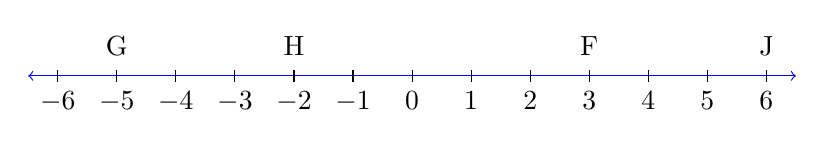
\begin{tikzpicture}[scale=0.75]
  % Draw horizontal line
  \draw[<->, blue] (-6.5,0) -- (6.5,0);
  % Draw ticks
  \foreach \x in {-6,...,6} {
    \draw (\x,0.1) -- (\x,-0.1) node[below] {$\x$};
  }
  % Add custom labels
  \node at (-5,0.5) {G};
  \node at (-2,0.5) {H};
  \node at (3,0.5) {F};
  \node at (6,0.5) {J};
\end{tikzpicture}
\end{figure}

The probability that selection falls in $HF$ is \pause $\frac{HF}{GH}=\frac{5}{11}$.
    \end{example}

    \pause 

    So in general, we draw the sample space and the set of desired outcomes as lines or line segments, and divide the length of the "desired outcomes" by the length of the "sample space" to get the probability.
    
\end{frame}



\begin{frame}{Geometric Probability}
   Imagine now that we are playing darts with two circles, and the smaller circle has two times smaller radius than the bigger one. 
    \begin{figure}
        \centering
        \includegraphics[width=0.3\linewidth]{Dart1.png}
        
        
    \end{figure}
    A dart is thrown at a random. What is the probability that it lands in the smaller circle? \pause

In this case, since the sample space and the set of desired outcomes is 2-dimensional, we should divide the \textit{area} of the smaller circle by the \textit{area} of the bigger circle.

The probability that the dart falls in the smaller circle, is $\frac{\pi r^2}{\pi (2r)^2}=\frac{1}{4}$.
    
    
\end{frame}


\begin{frame}{Geometric Probability}
One of the most powerful uses of geometric probability is applying it to problems that are not inherently geometric.

\pause \begin{example}
    Both the bus and you get to the bus stop at random times between 12 pm and 1 pm. When the bus arrives, it waits for 5 minutes before leaving. When you arrive, you wait for 20 minutes before leaving if the bus doesn't come. What is the probability that you catch the bus?
\end{example}

\pause Let $b$ denote the time that the bus arrives (after 12 pm), and $y$, the time you arrive. The set of all possible outcomes will be $[0,60]\times [0,60]$. \pause
\begin{figure}
    \centering
    \includegraphics[width=0.2\linewidth]{geom1.png}
    \end{figure}
    
    
\end{frame}


\begin{frame}{Geometric Probability}

Then, we need to determine the region of "success"; that is, the points where we catch the bus. Since the bus will wait for 5 minutes, you need to arrive within 5 minutes of the bus' arrival, so $y \le b+5$.
\begin{figure}
    \centering
    \includegraphics[width=0.2\linewidth]{geom2.png}
\end{figure}
    \pause
    However, you only wait for 20 minutes, so you can't arrive more than 20 minutes before the bus, so $y \ge b-20$.
\begin{figure}
    \centering
    \includegraphics[width=0.2\linewidth]{geom3.png}
\end{figure}
    
\end{frame}


\begin{frame}{Geometric Probability}

Combining our two conditions, we can draw the region of success:
\begin{figure}
    \centering
    \includegraphics[width=0.2\linewidth]{geom4.png}
\end{figure}
    \pause
    Now, we just need to find the area of this region. A simple method is to find the remaining area, and then subtract that from the total area:
\begin{figure}
    \centering
    \includegraphics[width=0.2\linewidth]{geom5.png}
\end{figure}
\pause
\begin{center}
    $\displaystyle\PP(\text{catching the bus})=\dfrac{60^2-\frac{55^2}{2}-\frac{40^2}{2}}{60^2}=\frac{103}{288}$
\end{center}
\end{frame}
\end{document}

